% =====================================================================================
% fig_explanation.tex: one prediction explained end to end (Q4; Notion E11).
%
% What the experiment tests: that the explanation of a single prediction can be read as
%   a short chain: class rule (head literals) -> prototypes it cites -> the matching nodes
%   in the input graph -> the trunk conditions on those nodes. Because the NMP+QAT
%   network computes exactly its rules, this chain IS the computation, not an
%   approximation of it.
% Plot: for one correctly predicted mutagen (and one non-mutagen, or one BAMultiShapes
%   graph): left, the graph with the nodes cited by the explanation highlighted; right,
%   the explanation tree (explorer/ "explanation tree"): class score = sum of true
%   literals >= threshold, each literal "graph has a node within t mismatches of Pk",
%   each Pk's cared bits as conditions. Constant literals greyed out / omitted
%   (evidence-only explanation).
% What it shows: what a user actually reads, and its length (e.g. 1-2 input-dependent
%   literals on Mutagenicity QAT fold 3).
% What it does not show: typical behaviour (one example; pick by a stated rule, e.g. a
%   random correctly classified test graph with seed, and add a failure case in the
%   appendix); readability of L1/L2 bits.
% Data: explorer export (python -m explorer export <run> --html) or SymbolicReader
%   (explorer/), final NMP+QAT fold of fig_prototypes.
% GENERATED BY: python plot_paper.py explanation   (sources: configs/paper_figures.yaml, code:
%   utils/paper_figures.py, branch feat/paper-figures). "preliminary: true" in the config
%   stamps PRELIMINARY on the figure; set it to false only when every source is final.
% STATUS: PRELIMINARY version drawn 2026-10-21 (qat_nmp, Mutagenicity test graph 5 of the representative fold). The head box lists constant literals too (use the evidence-only explanation), and the prototype box text overflows: needs a layout pass.
% TODO:
%   [ ] static export (SVG/PDF) of one explanation tree from explorer/ ->
%       paper/figures/fig_explanation.pdf.
% =====================================================================================
\begin{figure*}[t]
  \centering
  \IfFileExists{figures/fig_explanation.pdf}{%
    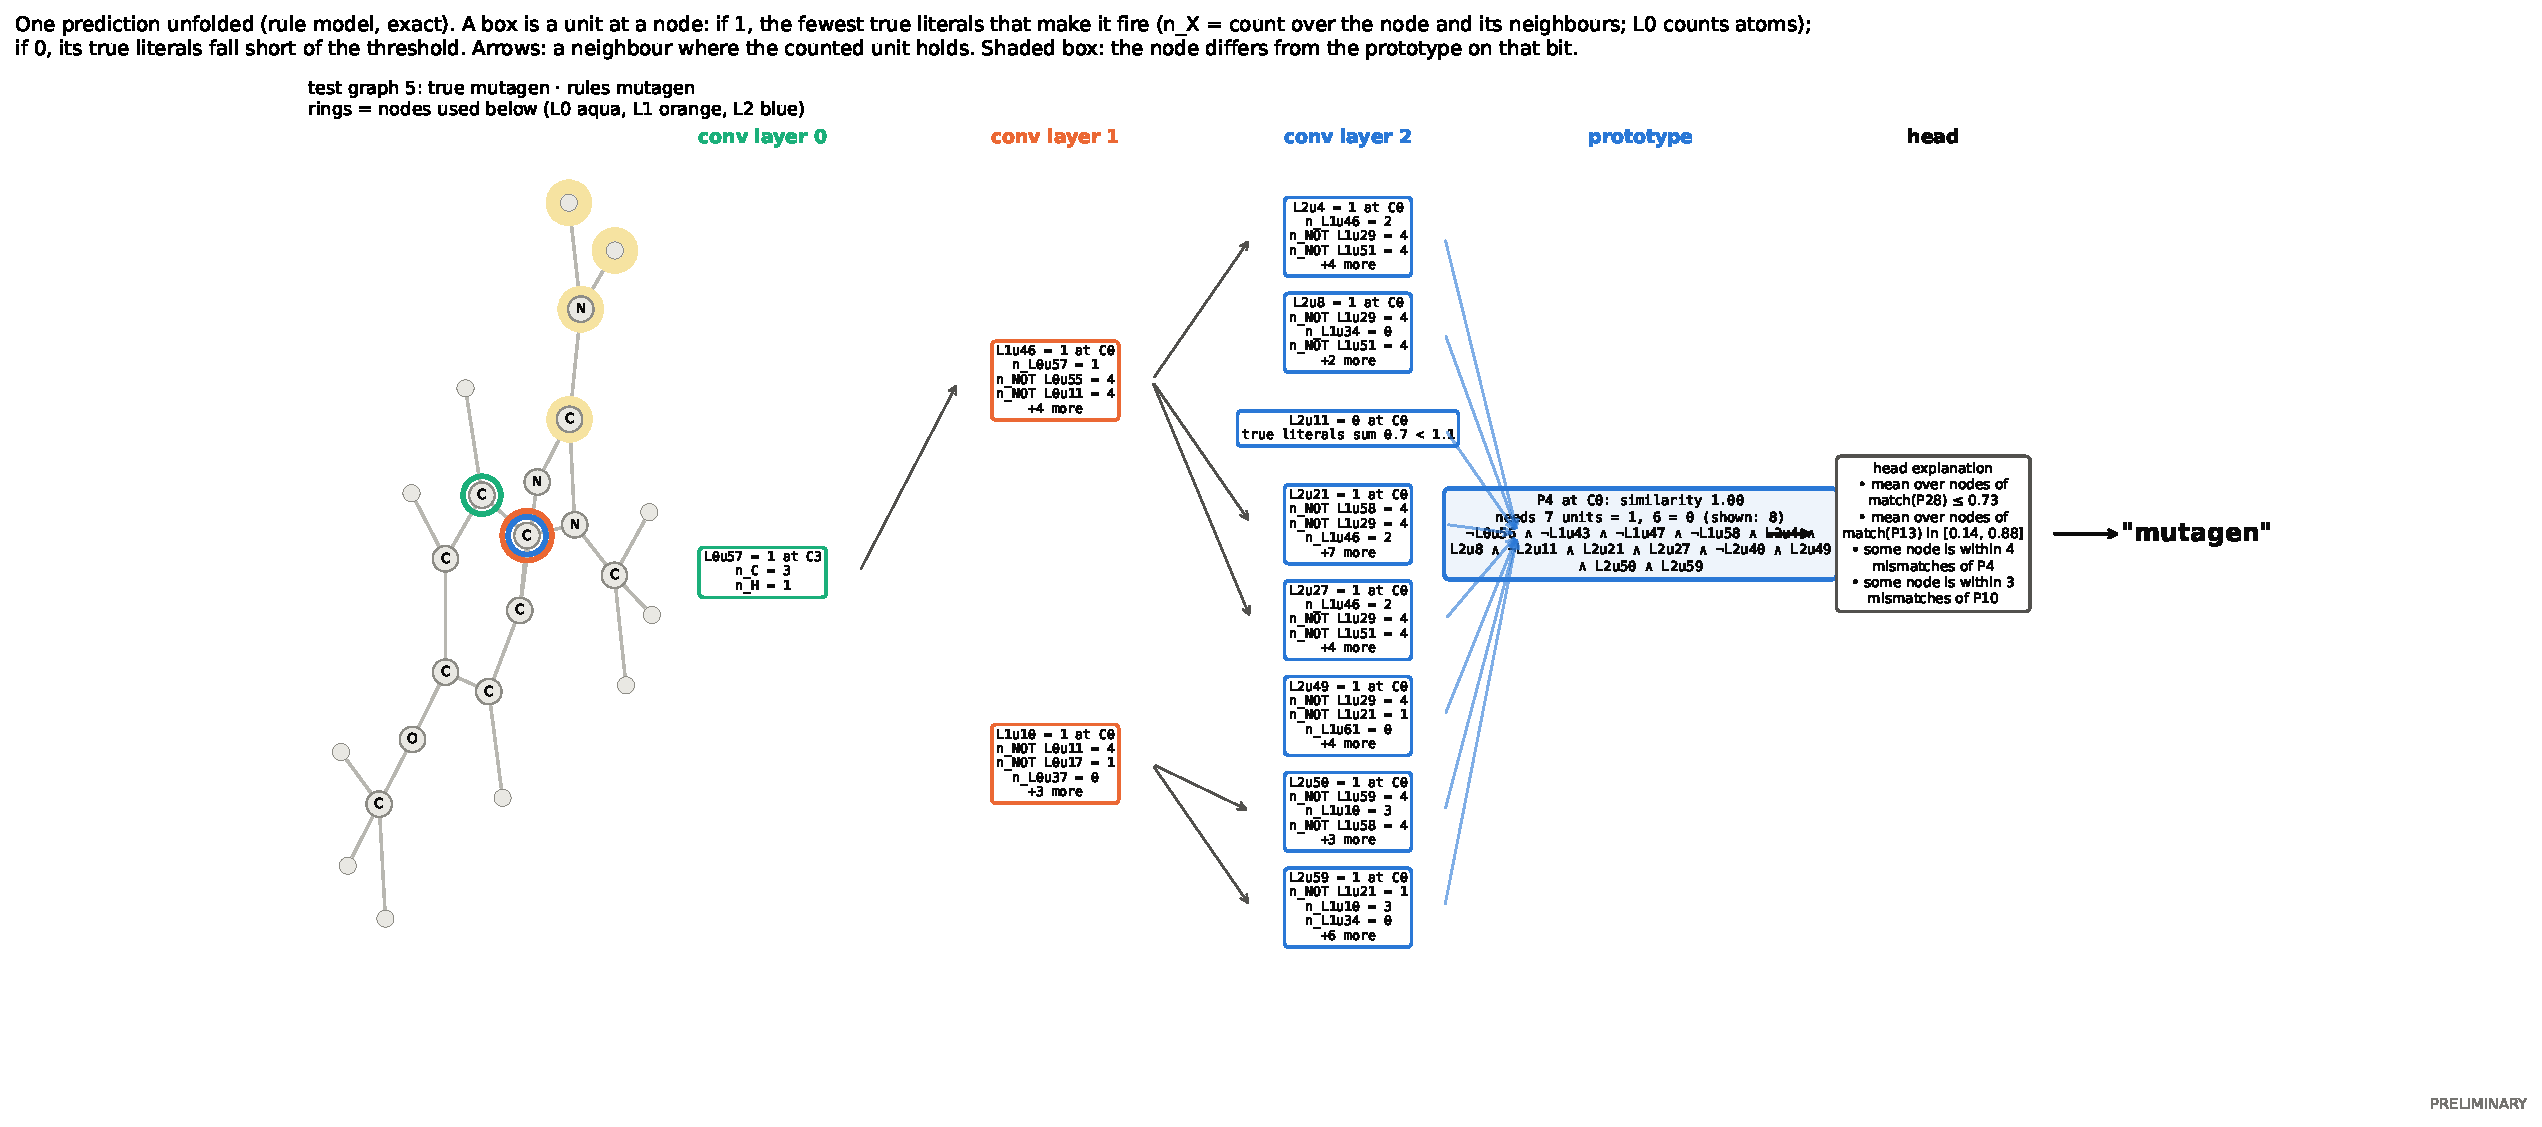
\includegraphics[width=\textwidth]{figures/fig_explanation.pdf}%
  }{\fbox{\parbox[c][5cm]{0.95\textwidth}{\centering\todo{fig\_explanation.pdf: one prediction explained}}}}
  \caption{Explanation of one test prediction on Mutagenicity. The class rule fires
    because the molecule contains nodes matching the cited prototypes (highlighted); each
    prototype is read as the trunk conditions it cares about. Since the network computes
    its rules exactly, this is the model's whole decision.}
  \label{fig:explanation}
\end{figure*}
